\documentclass[a4paper]{article}

\usepackage[T2A]{fontenc}
\usepackage[utf8]{inputenc}
\usepackage[ukrainian]{babel}
\usepackage{tikz}
\usepackage{lastpage} 
\usepackage[left=2.5cm, right=1.5cm, top=1.5cm, bottom=2.7cm]{geometry}
\usepackage{fancyhdr}
\usepackage{amsmath, amssymb, amstext} % Математичні символи
\usepackage{fp}
\usepackage{ragged2e}

\usepackage{listings}

\usepackage{xifthen} % Для умовних перевірок

% \usepackage{fontspec}
% \setmainfont{Times New Roman}

\usepackage{caption}


% \usepackage{graphicx}

\pagestyle{fancy}
\fancyhf{}
\renewcommand{\headrulewidth}{0pt}
\renewcommand{\footrulewidth}{0pt}

% \pagestyle{empty}

\newcommand{\makrosCalc}[1]{
    \FPeval{\the\fpresult}{#1}
}

\newcommand{\makrosmytitle}[2]{
    \thispagestyle{empty}
    \centering
    \textbf{Міністерство освіти і науки України}\\
    \textbf{КИЇВСЬКИЙ ПОЛІТЕХНІЧНИЙ УНІВЕРССИТЕТ}\\[2cm]
    \raggedleft
    Кафедра автоматизації та систем неруйнівного контролю\\
    Група ПМ-11
    \vfill
    \centering
    \textbf{ПРОЕКТУВАННЯ СИСТЕМ АВТОМАТИЗАЦІЇ}\\[1cm]
    \textbf{ЗВІТ З #1}\\[1cm]
    \textbf{\huge #2}
    \vfill
    \begin{flushleft}
        Керівник  \qquad\qquad\quad \hfill\qquad (підпис)\hfill 
        д.т.н., проф. Черепанська І. Ю.\\
        \hfill (дата)\\[2cm]
        Виконавець\hfill (підпис)\hfill Юша Володимир Ігорович\\
        \hfill (дата)
    \end{flushleft}
    \vfill
    \centering
    2025
}

\newcommand{\makrosFrameBig}[2]{
    \thispagestyle{empty} % Вимикає номер сторінки на першій сторінці
    
    \begin{tikzpicture}[remember picture, overlay]
        \begin{scope}[shift={([xshift = 20 mm, yshift = 10 mm]current page.south west)}]
            \draw[line width=2] (0,0) rectangle (180 mm,277 mm);
        \end{scope}
    \end{tikzpicture}
    
    \begin{tikzpicture}[remember picture, overlay]
        \begin{scope}[shift={([xshift = 20 mm, yshift = 10 mm]current page.south west)}, x=1mm, y=1mm]
            \draw[line width=2] (0,0) rectangle (180,40);
            \draw[line width=2]  (7,40) -- (7, 25);
            \draw[line width=2] (17,40) -- (17, 0);
            \draw[line width=2] (40,40) -- (40, 0);
            \draw[line width=2] (55,40) -- (55, 0);
            \draw[line width=2] (65,40) -- (65, 0);
            \draw[line width=2] (135,25) -- (135,0);
            \draw[line width=2] (140,15) -- (140,20);
            \draw[line width=2] (145,15) -- (145,20);
            \draw[line width=2] (150,25) -- (150,15);
            \draw[line width=2] (165,25) -- (165,15);
        
            \draw (0,35) -- (65, 35);
            \draw[line width=2] (0,30) -- (65, 30);
            \draw[line width=2] (0,25) -- (180, 25);
            \draw (0,20) -- (65, 20);
            \draw (0,15) -- (65, 15);
            \draw (0,10) -- (65, 10);
            \draw (0,5) -- (65, 5);
        
            \draw[line width=2] (135,20) -- (180, 20);
            \draw[line width=2] (135,15) -- (180, 15);
            
            \node at (3.5, 27.5) {Зм.};
            \node at (12, 27.5) {Лист};
            \node at (28.5, 27.5) {№ докум.};
            \node at (47.5, 27.5) {Підпис};
            \node at (60, 27.5) {Дата};
            
            \node at (7, 22.5) {Розроб.};
            \node at (6.5, 17.5) {Перев.};
            \node at (8.5, 7.5) {Н. Контр.};
            \node[align=left] at (5, 2.5) {Затв.};
            
            \node at (142.5, 22.5) {Літ.};
            \node at (157.5, 22.5) {Аркуш};
            \node at (172, 22.5) {Аркушів};
        
            \node[align=left, font=\itshape, anchor=south west, scale=0.9] at (16, 20) {Юша В. І.};
            \node[align=left, font=\itshape, anchor=south west, scale=0.8] at (16, 15) {Черепанська І.Ю.};
            \node[align=left, font=\itshape, anchor=south west, scale=0.8] at (16, 0) {Черепанська І.Ю.};
        
            \node[anchor=center, font=\itshape, scale=1.5] at (122, 32) {#1};
            \node[align=center, font=\itshape, anchor=center] at (100, 12) {#2};
            \node[align=left, font=\itshape, anchor=south west, scale=0.9] at (135, 5) {КПІ ім. І. Сікорського, ПБФ};
            \node[anchor=center, font=\itshape] at (158, 17) {2};
            \node[anchor=center, font=\itshape] at (172, 17) {\pageref{LastPage}};    
        \end{scope} 
    \end{tikzpicture}
}

\newcommand{\makrosFrameSmall}[1]{
    % \thispagestyle{empty} % Вимикає номер сторінки на першій сторінці
    
    \begin{tikzpicture}[remember picture, overlay]
        \begin{scope}[shift={([xshift = 20 mm, yshift = 10 mm]current page.south west)}]
            \draw[line width=2] (0,0) rectangle (180 mm,277 mm);
        \end{scope}
    \end{tikzpicture}
    
    \begin{tikzpicture}[remember picture, overlay]
        \begin{scope}[shift={([xshift = 20 mm, yshift = 10 mm]current page.south west)}, x=1mm, y=1mm]
            \draw[line width=2] (0,0) rectangle (180,15);
            \draw[line width=2] (7,0) -- (7, 15);
            \draw[line width=2] (17,0) rectangle (43,15);
            \draw[line width=2] (55,0) rectangle (64,15);
            \draw[line width=2] (170,0) -- (170, 15);

            \draw[line width=2] (0,5) -- (64, 5);
            \draw               (0,10) -- (64, 10);
            \draw[line width=2] (170,8) -- (180, 8);

            \node[anchor=center, scale=0.8] at (3.5, 2.5) {Змн.};
            \node[anchor=center, scale=0.9] at (12, 2.5) {Арк.};
            \node[anchor=center] at (30, 2.5) {№~докум.};
            \node[anchor=center, scale=0.9] at (49, 2.5) {Підпис};
            \node[anchor=center, scale=0.9] at (59, 2.5) {Дата};
            \node[anchor=center, font=\itshape, scale=1.5] at (115, 7.5) 
                {#1};
            \node[anchor=center] at (175, 12) {Арк.};
            \node[anchor=center] at (175, 4) {\thepage};
            
        \end{scope}
    \end{tikzpicture}
}

% % \makrosLab{1}{Шифр}{Назва}
% \newcommand{\makrosLab}[3]{ 
%     \fancyfoot[C]{\makrosFrameSmall{#2}}
%     \ifthenelse{\equal{#2}{л}}%    
%     % \makrosmytitle{#1}{#3}
%     \newpage
%     \makrosFrameBig{#2}{#3}
%     \justify
%     \fontsize{14}{16}\selectfont
%     \section*{Лабораторна робота №#1}
% }

% Оголошуємо змінні
\newcommand{\mytitlegenitive}{}
\newcommand{\mytitle}{}
\newcommand{\shyfr}{}

% \makrosLab{номер}{п чи л}{Назва}
\newcommand{\makrosLab}[3]{ 


    % Перевіряємо другий аргумент
    \ifthenelse{\equal{#2}{л}}%
        {
            \renewcommand{\mytitle}{Лабораторна робота №#1}
            \renewcommand{\mytitlegenitive}{ЛАБОРАТОРНОЇ РОБОТИ №#1}
            \renewcommand{\shyfr}{ПМ1115.04.00.0#1 ЛР}
        }%
        { \ifthenelse{\equal{#2}{п}}%
            {
                \renewcommand{\mytitle}{Практична робота №#1}
                \renewcommand{\mytitlegenitive}{ПРАКТИЧНОЇ РОБОТИ №#1}
                \renewcommand{\shyfr}{ПМ1115.04.00.0#1 ПР}
            }%
            {\section*{ПОМИЛКА}}%
        }%

    % Використання змінних
    \fancyfoot[C]{\makrosFrameSmall{\shyfr}}
    \makrosmytitle{\mytitlegenitive}{#3}
    \newpage
    \makrosFrameBig{\shyfr}{#3}
    \justifying
    \vspace*{-20mm}
    \fontsize{14}{16}\selectfont
    \section*{\mytitle}
}



\begin{document}
    \makrosLab{4}{л}{
Дослідження використання Arduino в \\
автоматизованих системах контролю\\ 
та розробка програмного забезпечення\\
для мікроконтролерів.
    }
\section*{Тема роботи}
Вивчення можливостей використання платформи Arduino у складі систем автоматичного контролю технологічних параметрів. Розробка алгоритмічно-програмного забезпечення роботи мікроконтролерів в системах автоматизації на прикладі платформи Arduino.

\section*{Мета роботи}
Вивчити будову, принцип дії та основні характеристики мікроконтролерів на прикладі мікроконтролера ATmega328 платформи Arduino Uno, навчитися підключати до них зовнішні пристрої та засоби автоматизації, вимірювальні пристрої тощо, а також розробляти, завантажувати та налагоджувати алгоритмічно-програмне забезпечення їх роботи.


\section*{Обладнання та інструменти}
\begin{itemize} 
    \item Arduino Uno R3 на базі мікроконтролера ATmega328.
    \item Гребінка 40 Pin 1x40, однорядна.
    \item Персональний комп’ютер.
    \item Програмне забезпечення для роботи з платформою Arduino.
    \item Датчики температури.
    \item З’єднувальні провідники.
\end{itemize}

\newpage

\section*{Програма миготіння світлодіодом}

Завдання: модифікувати скетч Blink у Blink2 та
Blink3, зменшивши в 2 та збільшивши у 3 рази відповідно
затримку мерехтіння користувацького світлоліода L.

\begin{lstlisting}[language=C++, caption=Програма Blink2 - вбудований світлодіод миготить у 2 рази швидше]
void setup() {
  pinMode(LED_BUILTIN, OUTPUT);
}

void loop() {
  digitalWrite(LED_BUILTIN, !digitalRead(LED_BUILTIN));
  delay(500/2);
}
\end{lstlisting}


\begin{figure}[h]
    \centering
    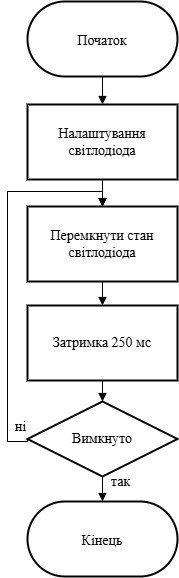
\includegraphics[width=0.25\textwidth]{imgs/LW4.0.1.drawio.png}
    \caption*{Рис. 4.1: Діаграма миготіння Blink2}
\end{figure} 

\newpage

\begin{lstlisting}[language=C++, caption=Програма Blink3 - вбудований світлодіод миготить у 3 рази повільніше]
void setup() {
  pinMode(LED_BUILTIN, OUTPUT);
}

void loop() {
  digitalWrite(LED_BUILTIN, !digitalRead(LED_BUILTIN));
  delay(500*3);
}
\end{lstlisting}

\begin{figure}[h]
    \centering
    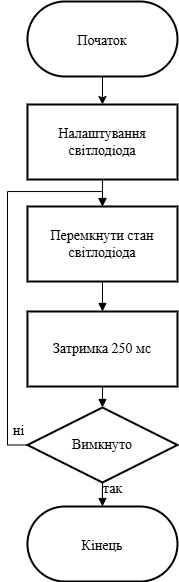
\includegraphics[width=0.3\textwidth]{imgs/LW4.0.2.drawio.png}
    \caption*{Рис. 4.2: Діаграма миготіння Blink3}
\end{figure} 

\newpage 


% https://wokwi.com/projects/425977612553598977


\section*{Код програми}
\begin{lstlisting}[language=C++, caption=Програма для вимірювання температури]
const int BETA = 3950;

void setup() {
  Serial.begin(9600);
  Serial.println("valueSensor\t\u2103");
}

void loop() {
  int valueSensor  = analogRead(A0);
  float celsius = 1 / (log(1 / (1023. / valueSensor - 1)) /
                  BETA + 1.0 / 298.15) - 273.15;
  Serial.println(String(valueSensor)+"\t"+String(celsius));
  delay(500);
}
\end{lstlisting}

\subsection*{Алгоритм роботи програми}
\begin{enumerate}
    \item Ініціалізується серійний порт для обміну даними з комп'ютером через USB.
    \item Виводиться заголовок стовпців у серійному моніторі.
    \item У нескінченному циклі (\texttt{loop()}):
    \begin{enumerate}
        \item Зчитується аналогове значення з датчика температури на вході A0.
        \item Виконується перетворення аналогового значення у температуру за допомогою формули з використанням коефіцієнта BETA.
        \item Виводиться у серійний порт значення сенсора та розрахована температура у градусах Цельсія.
        \item Виконується затримка у 500 мс перед наступним зчитуванням значень.
    \end{enumerate}
\end{enumerate}

\begin{figure}[h]
    \centering
    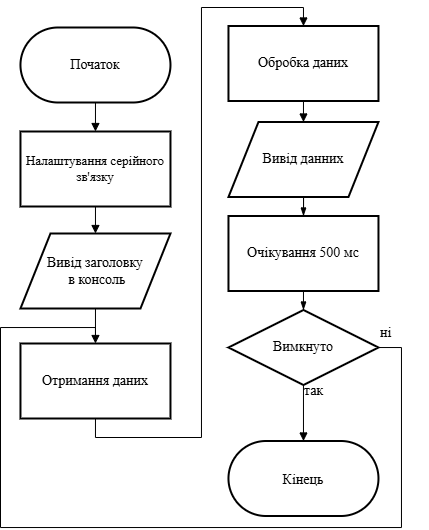
\includegraphics[width=0.8\textwidth]{imgs/LW4.01.drawio.png}
    \caption*{Рис. 4.3: Діаграма алгоритму роботи програми вимірювання температури}
\end{figure} 

\section*{Результати вимірювання}
\begin{enumerate}
    \item Вимірювання температури проводилися симуляьорі.
    \item Значення, отримані з термістора, були в межах 0-1023.
\end{enumerate}

\begin{figure}[h]
  \centering
  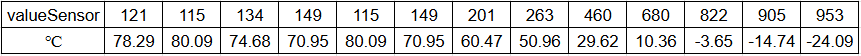
\includegraphics[width=1\textwidth]{imgs/LW4.2.png}
  \caption*{Рис. 4.4: Таблиця результатів вимірювання}
\end{figure} 


\begin{figure}[h]
  \centering
  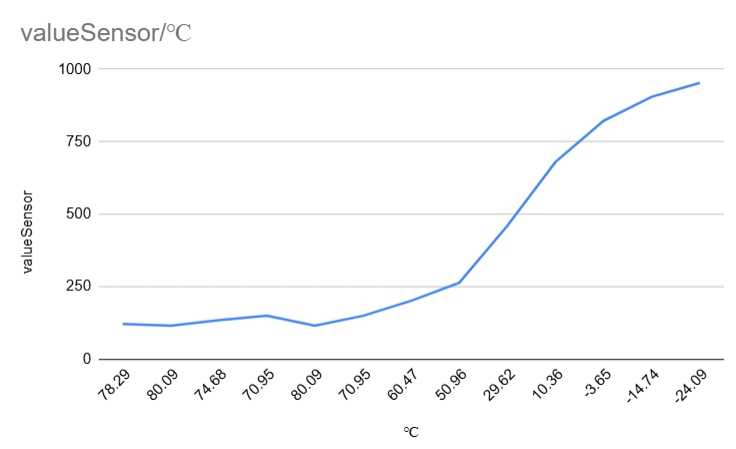
\includegraphics[width=0.8\textwidth]{imgs/LW4.3.png}
  \caption*{Рис. 4.5: Діаграма результатів вимірювання}
\end{figure} 

% \newpage

\section*{Висновки}
В ході виконання лабораторної роботи було вивчено принцип роботи мікроконтролера ATmega328 на платформі Arduino Uno, встановлено та налаштовано програмне середовище Arduino IDE, а також реалізовано програму для вимірювання температури за допомогою датчика.

\section*{Відповіді на контрольні питання}
\begin{enumerate}
    \item Платформа Arduino — це апаратно-програмний комплекс, що складається з мікроконтролерів та середовища програмування для розробки автоматизованих систем.
    \item Основні компоненти плати Arduino: мікроконтролер, роз'єми живлення, USB-інтерфейс, цифрові та аналогові входи/виходи, світлодіоди індикації, кварцовий генератор, кнопка скидання.
    \item Мова програмування Arduino базується на C/C++ та містить бібліотеки для роботи з апаратними компонентами.
    \item Основні компоненти програмного забезпечення: середовище розробки Arduino IDE, бібліотеки для роботи з периферійними пристроями, компілятор та засоби завантаження коду на плату.
\end{enumerate}


    
\end{document}